\section{How to Get There}

CCSS will be held at the UVM Grossman School of Business (Ifshin Hall) in the Keller Room (Ifshin 107). The Business School is located at 55 Colchester Ave, Burlington, VT 05405.

The most natural entrance to the Keller room is illustrated with the "X" marker below:

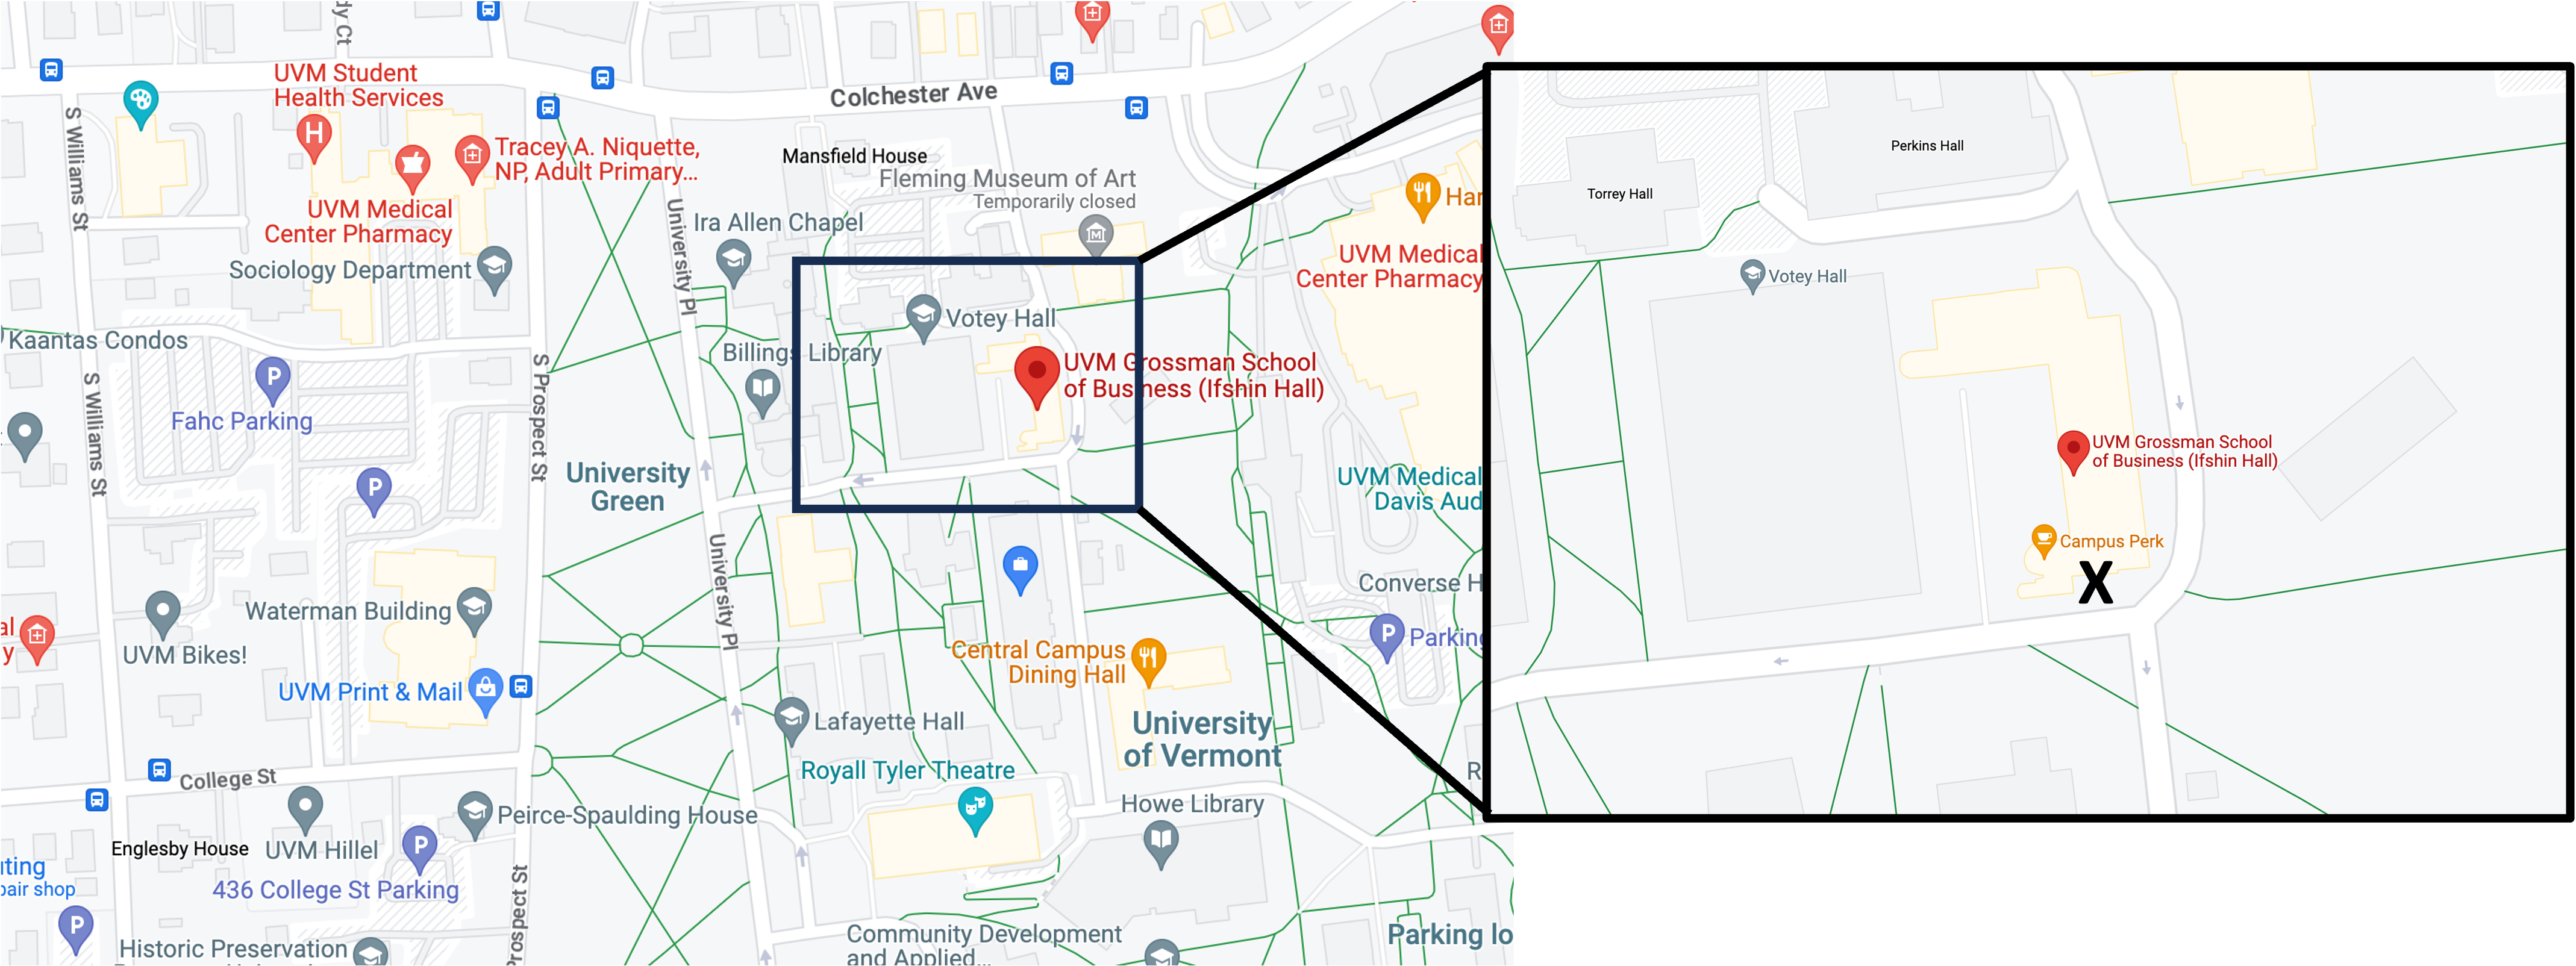
\includegraphics[width=\textwidth]{images/map.png}


\section{Food Recommendations}

\subsection{Breakfast}

\begin{itemize}
    \item Willow's Bagels: allergy friendly options, order ahead to beat the line
    \item The Café Hot: Vegetarian breakfast sandwiches, donuts
    \item The Skinny Pancake: The creperie chain of Vermont
    \item Black Cap: Nice sandwiches, scones, and coffee.
\end{itemize}

\subsection{Lunch}

\begin{itemize}
    \item Folino's: Sourdough, wood-fired pizza
    \item Top of the block: Sandwiches/soup/salad
    \item Zabby's: Buffet by weight
    \item Pokeworks: Poke bowl fast food
    \item Pingala Cafe: Vegan food and not too far
    \item El Cortijo: Taqueria in a small vintage diner
    \item Masala Elaichi: Indian food and pretty close to campus
    \item Four Corners of the Earth: Legendary if you can wait a while
    \item Davis Center: Closest option with standard soup/sandwich options
    \item Kampus Kitchen: Sandwiches in a convenience store pretty close to campus
\end{itemize}

\subsection{Dinner}

\begin{itemize}
    \item Folino's (Yep, it's good.)
    \item Citizen Cider: Lots of allergy friendly options
    \item Sherpa Kitchen: Nepalese food
    \item American Flatbread: Small New England wood-fired pizza chain
    \item Istanbul Kebab House: Turkish Mediterranean food
\end{itemize}

\subsection{After Dinner}

\begin{itemize}
    \item Burlington Bay: Creemees
    \item Little Gordo Creemee Stand: Self-explanatory
    \item Wallflower Collective: Bar right next to Folino's
    \item JP's: The place to go for foosball and Karaoke
\end{itemize}
